\chapter{The jSCAPE System}

The jSCAPE system is designed for two distinct groups of users: students and teachers/lecturers. This separation of roles lead to the development of the main application for students, and an administrator tool for teachers/lecturers.

\begin{figure}[H]
\centering
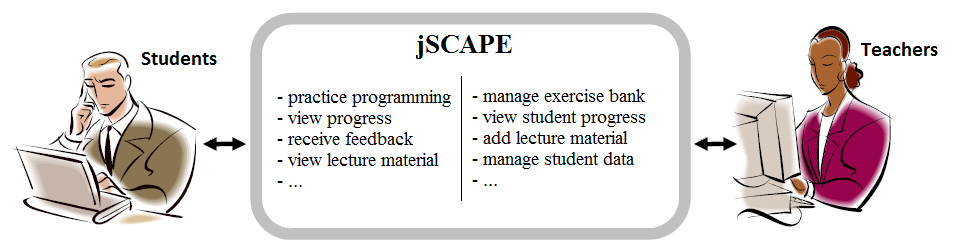
\includegraphics[width=\textwidth,height=\textheight,keepaspectratio]{jscape_use_case}
\caption{Use case diagram of the jSCAPE system.}
\label{fig:jscape_use_case}
\end{figure}

Figure \ref{fig:jscape_use_case} shows some of the main capabilities of the jSCAPE system. Students can practice their understanding of programming concepts by answering exercises provided by the lecturers, and receive feedback while doing so. In addition, students can track their progress by viewing various graphs and charts of their performance on particular exercise categories. Finally, students can access lecture notes and website links provided by the teacher. \newline

Teachers can manage the exercise bank, whether it be adding exercises manually or automatically generating new ones based on templates. They can keep track of their students' progress and thereby identify any difficulties particular students are having. Finally, teachers are responsible for adding lecture material, website links and creating student profiles to store in the database.\newline

In the rest of this chapter we take a closer look at the current available features of jSCAPE.\newline

At the time of writing this report, we would like to note that the screen shots of the application do not represent the final version of jSCAPE, in particular, the graphics and logos haven't been finalized.

\section{Student view}

\subsection{Login screen}
\begin{figure}[H]
\centering
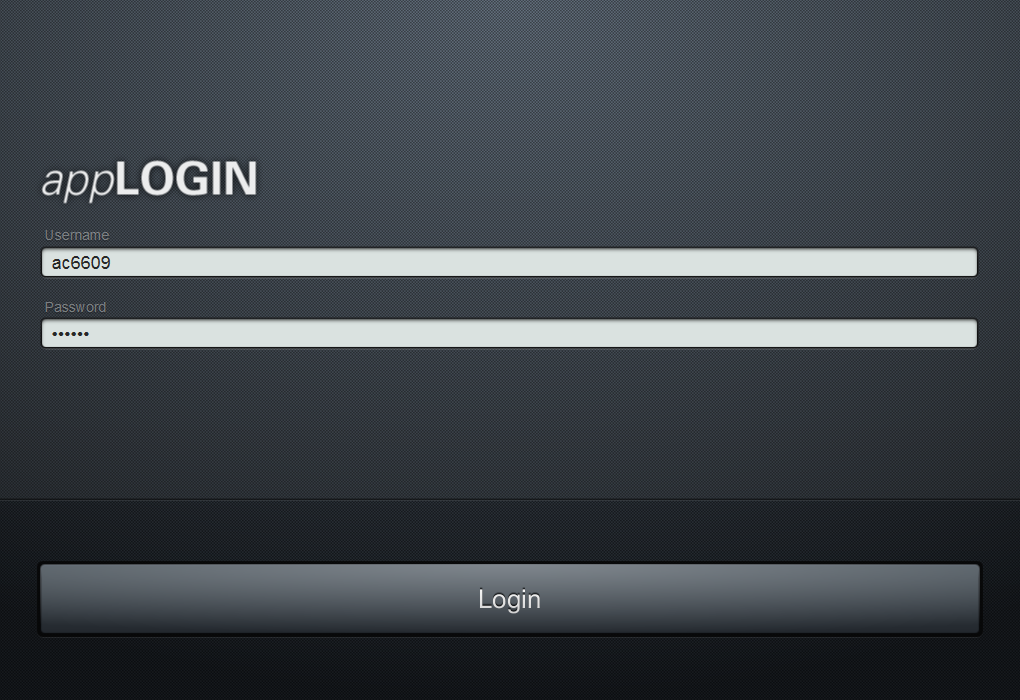
\includegraphics[scale=0.45]{login_screen}
\caption{The jSCAPE login screen.}
\label{fig:login_screen}
\end{figure}

For a student to use jSCAPE, they need to be in possession of login credentials, usually acquired by asking the appropriate teacher or lecturer. A connection to the jSCAPE system will be rejected if the entered login details are incorrect. Otherwise, the student can proceed to jSCAPE and access its features.

\subsection{Tracking progress through statistical data}
\label{subsec:tracking-progress}
After a successful login the student lands on the Profile tab which presents information about the student, as well as statistical data on the student's performance and usage of the system.

\begin{figure}[H]
\centering
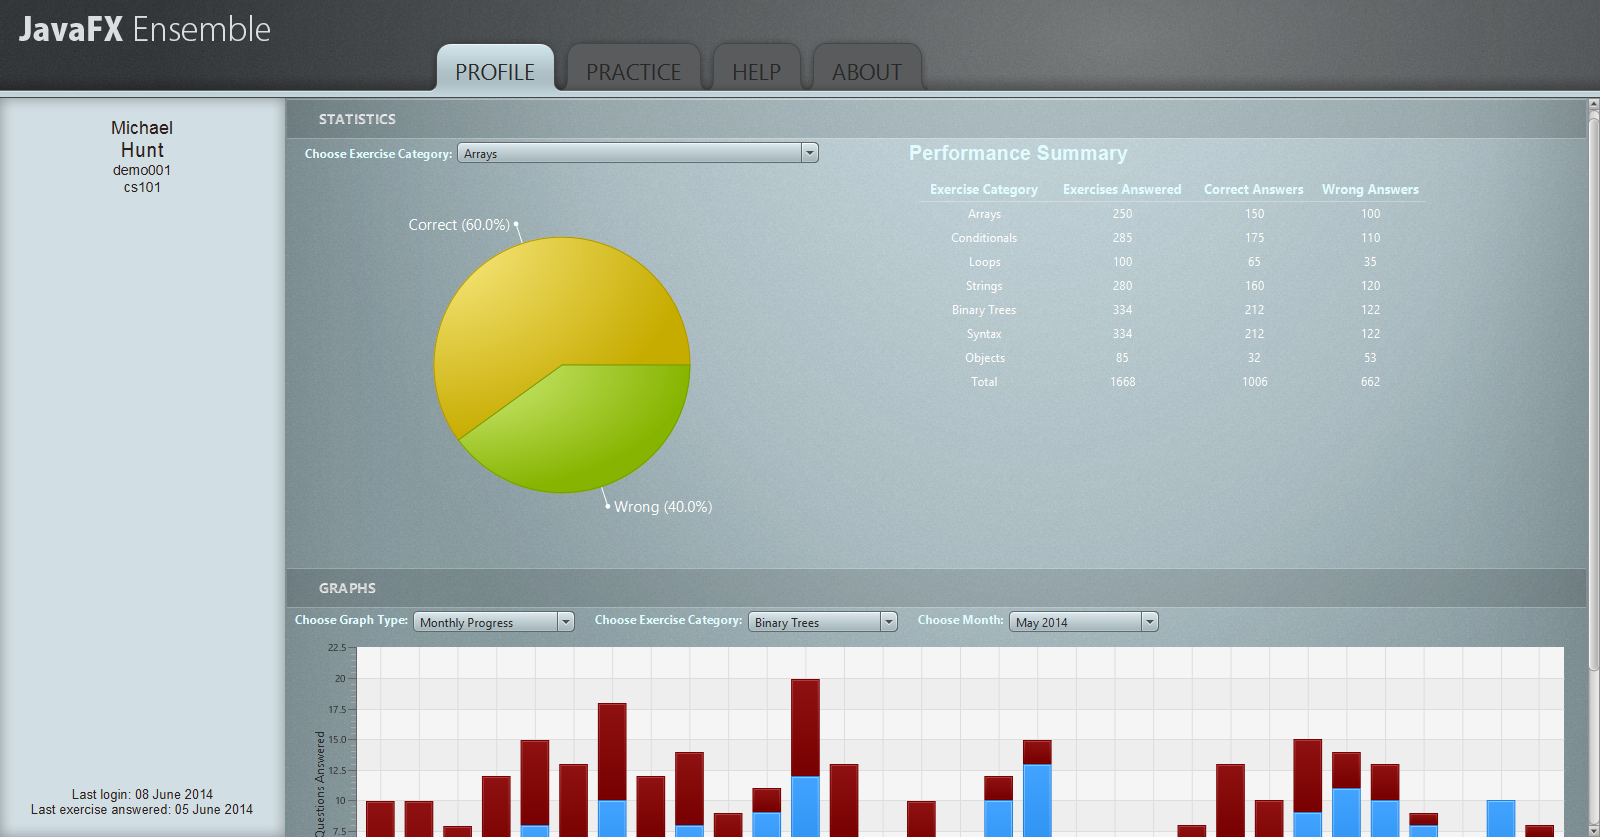
\includegraphics[width=\textwidth,height=\textheight,keepaspectratio]{profile_screen_overview}
\caption{An overview of the Profile tab in jSCAPE.}
\label{fig:profile_screen_overview}
\end{figure}

Figure \ref{fig:profile_screen_overview} shows the Profile tab after the student has logged in to the system. Profile information for the student is listed on the left hand side, in the light-blue rectangle. This information includes the student's first name, last name, user name, which class the student is in, the last time the student logged in, and the last time the student answered an exercise. \newline

The main part of the Profile tab is split horizontally between statistical data in the form of pie charts and tables, and graphical data in the form of bar charts.

\begin{figure}[H]
\centering
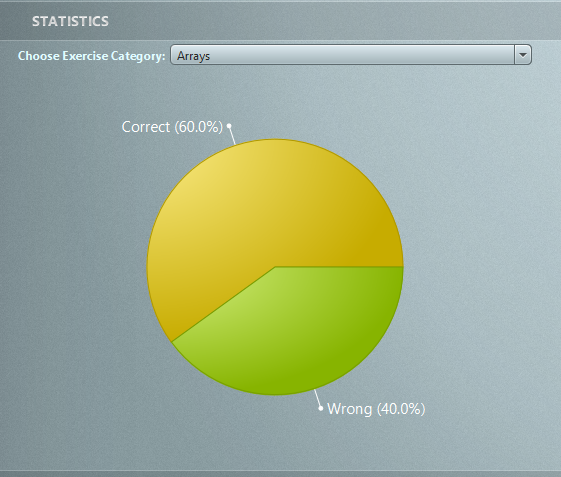
\includegraphics[scale=0.6]{pie_chart_stats}
\caption{Pie chart statistics for exercise category.}
\label{fig:pie_chart_stats1}
\end{figure}

Figure \ref{fig:pie_chart_stats1} shows the performance of the student in a particular exercise category, in this case ``Arrays". In the example, the student has gotten 60\% of array exercises correct and thus 40\% of them wrong. The student can view the performance pie chart for other exercise categories by changing the selected category in the combo box.

\begin{figure}[H]
\centering
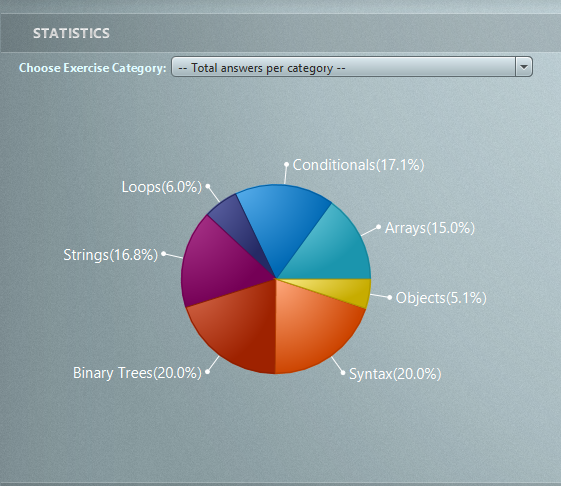
\includegraphics[scale=0.7]{pie_chart_stats2}
\caption{Pie chart statistics for distribution of answers.}
\label{fig:pie_chart_stats2}
\end{figure}

Another type of pie chart available in jSCAPE can be seen in figure \ref{fig:pie_chart_stats2}. This pie chart shows the distribution of answers per exercise category. This is a useful feature when a student is trying to get a balanced amount of practice in all exercise categories. \newline

Next, performance data is presented to the student in the performance summary table, shown in figure \ref{fig:performance_summary}. In this table, there is a row for every exercise category and a row for the total of each column. Each row contains the number of exercises answered, the number of correct answers and the number of wrong answers associated with a particular exercise category.

\begin{figure}[H]
\centering
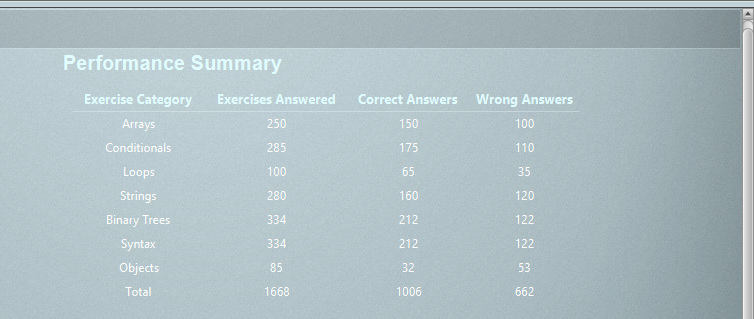
\includegraphics[width=\textwidth,height=\textheight,keepaspectratio]{performance_summary}
\caption{Performance summary table.}
\label{fig:performance_summary}
\end{figure}

In the lower half of the Profile tab there is the possibility to view performance data in the form of stacked bar charts.

\begin{figure}[H]
\centering
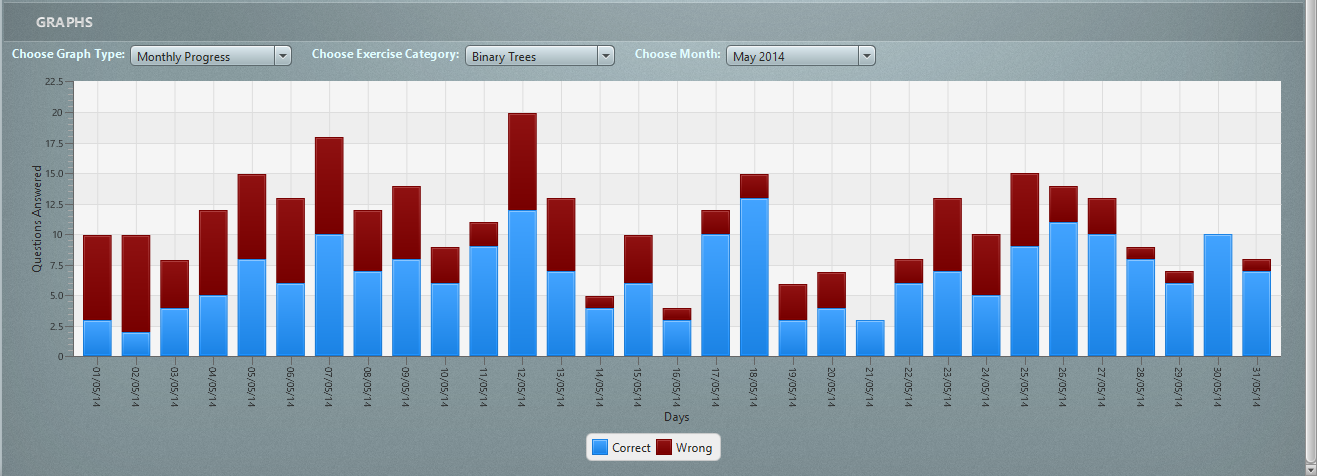
\includegraphics[width=\textwidth,height=\textheight,keepaspectratio]{monthly_progress}
\caption{Graph data of monthly progress.}
\label{fig:monthly_progress}
\end{figure}

Figure \ref{fig:monthly_progress} shows the monthly progress of a student for the month of May 2014 and for the exercise category ``Binary Trees". The number of correct answers (in blue) and wrong answers (in red) are graphed for each day where the student answered exercises. The student can view his monthly progress in other exercise categories and other months by manipulating the appropriate combo boxes. This historical data goes back to the first month in which the student answered an exercise.

\begin{figure}[H]
\centering
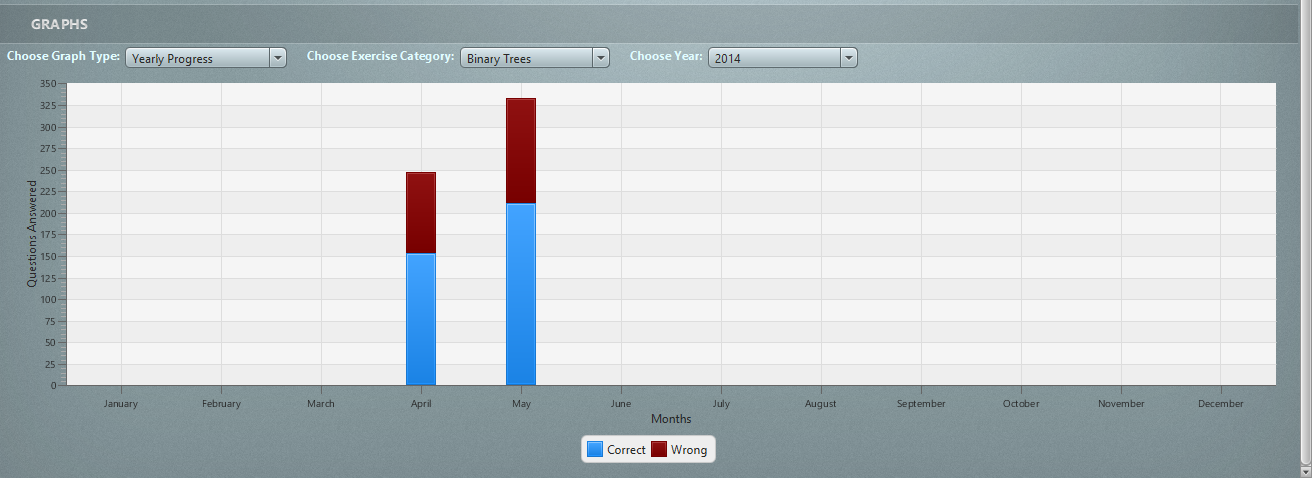
\includegraphics[width=\textwidth,height=\textheight,keepaspectratio]{yearly_progress}
\caption{Graph data of yearly progress.}
\label{fig:yearly_progress}
\end{figure}

Figure \ref{fig:yearly_progress} shows the yearly progress of a student in 2014 for the exercise category ``Binary Trees". For each month where the student answered exercises, a stacked bar can be found containing the total number of correct answers (in blue) and the total number of wrong answers (in red) for that particular year and exercise category. The student can view his yearly progress in other exercise categories and other years by manipulating the appropriate combo boxes. This historical data goes back to the year in which the student first started answering exercises.

\subsection{Practicing programming}
%show difficulty progression of exercises
\begin{figure}[H]
\centering
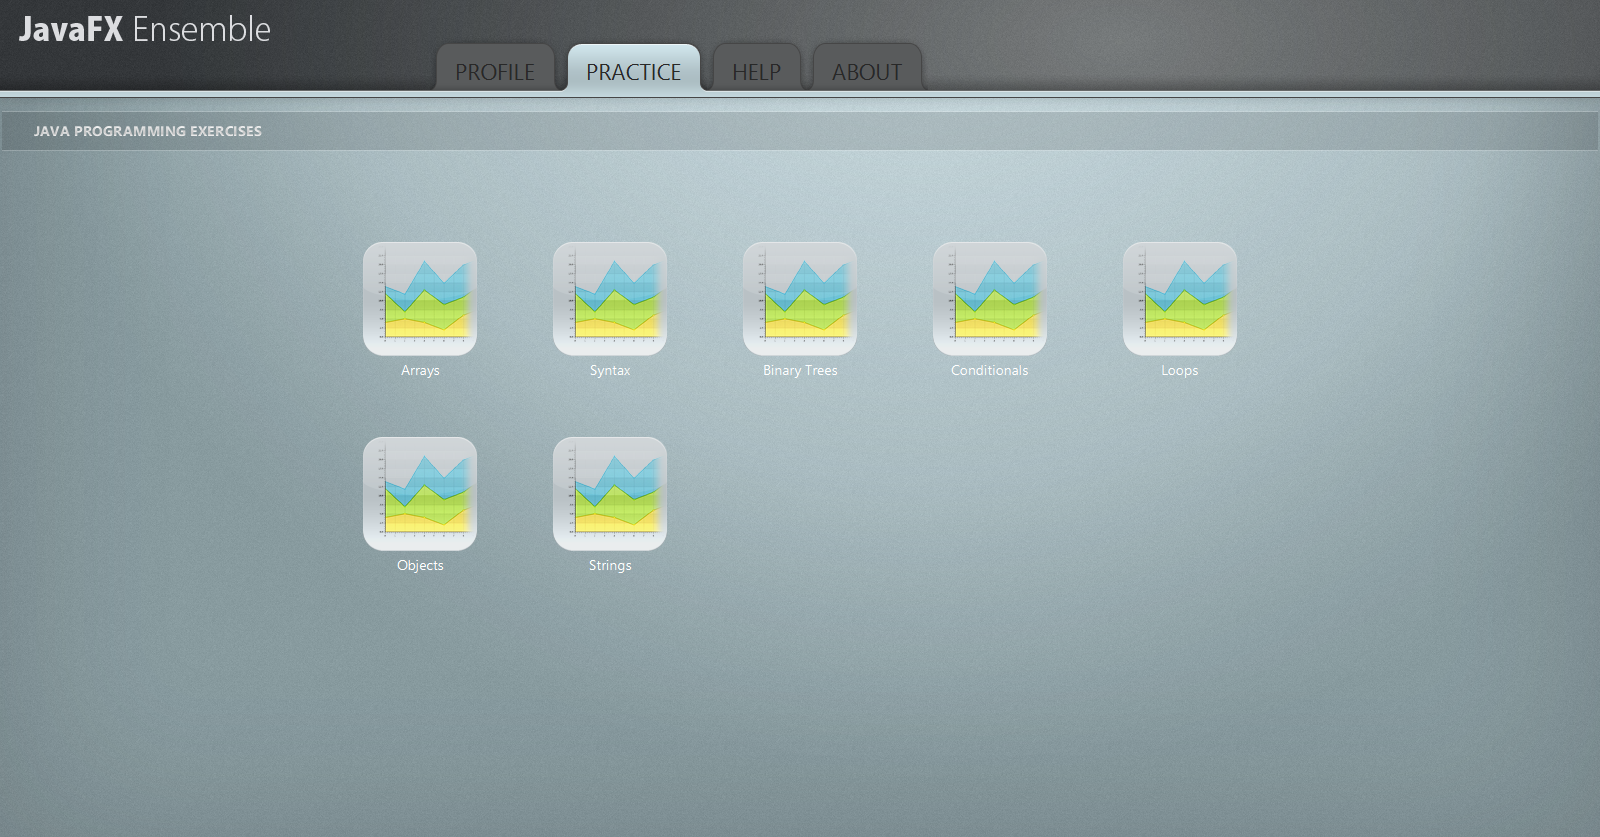
\includegraphics[width=\textwidth,height=\textheight,keepaspectratio]{practice_overview}
\caption{An overview of the Practice tab in jSCAPE.}
\label{fig:practice_overview}
\end{figure}

\begin{figure}[H]
\centering
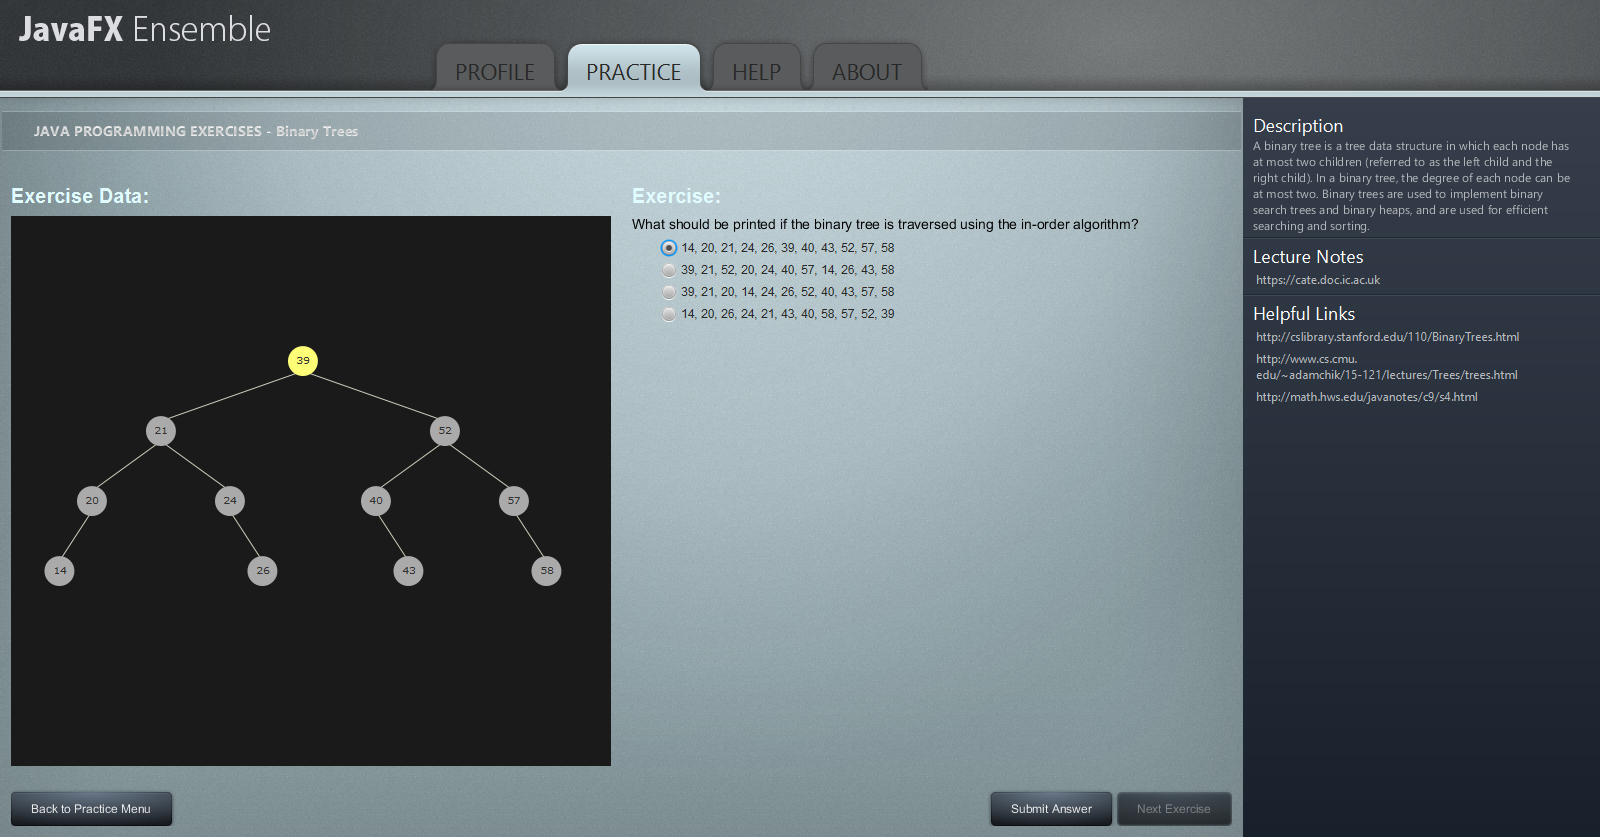
\includegraphics[width=\textwidth,height=\textheight,keepaspectratio]{practice_binary_trees}
\caption{The Practice tab view showing an exercise on binary trees.}
\label{fig:practice_binary_trees}
\end{figure}

\begin{figure}[H]
\centering
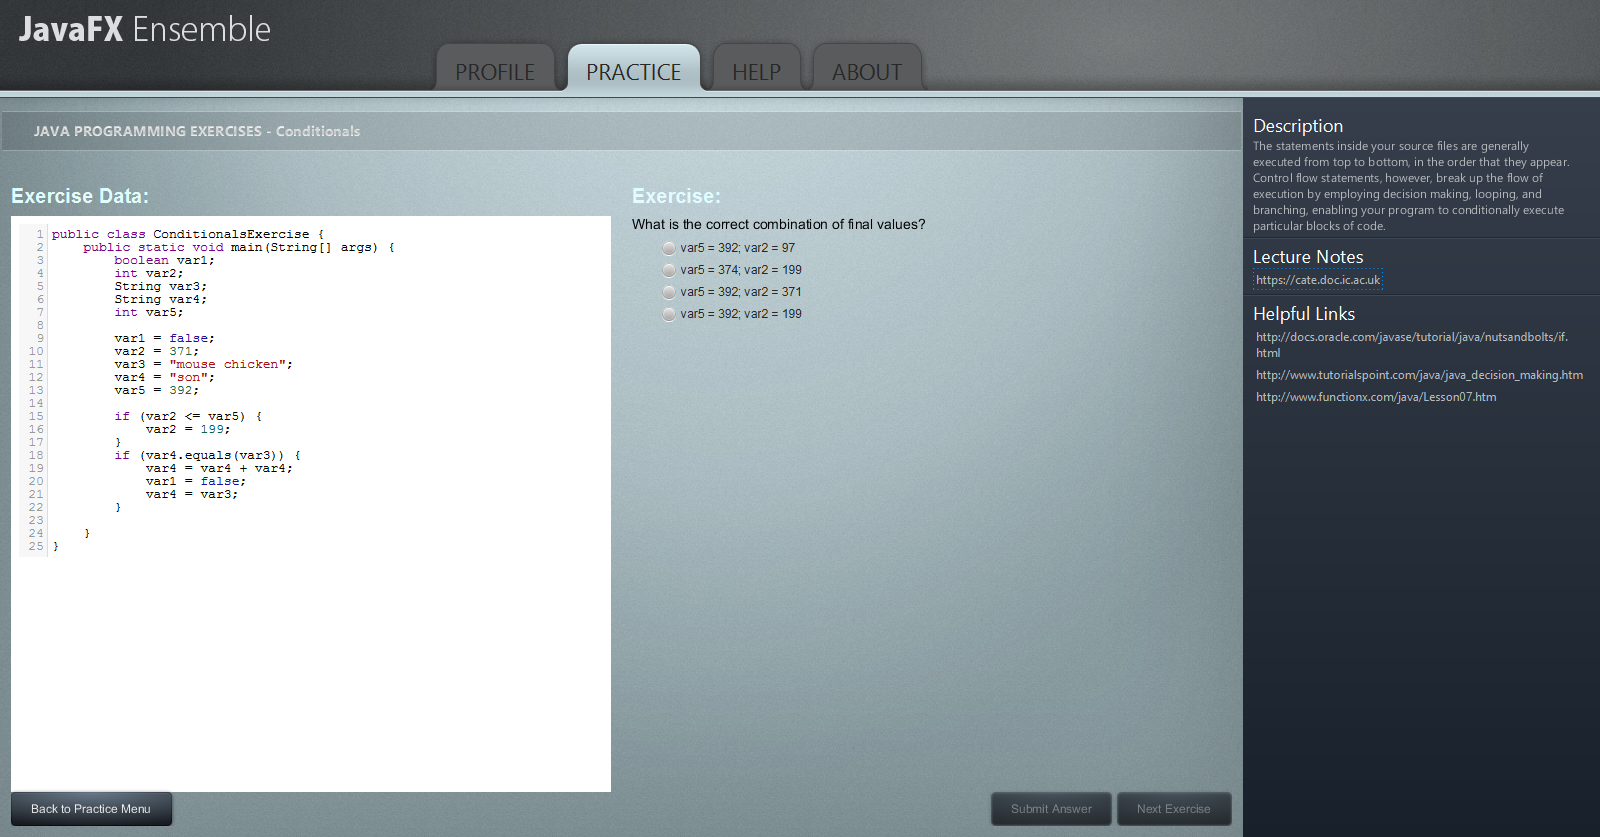
\includegraphics[width=\textwidth,height=\textheight,keepaspectratio]{practice_conditionals}
\caption{The Practice tab view showing an exercise on conditionals.}
\label{fig:practice_conditionals}
\end{figure}


\section{Teacher view}
The teacher's main access to the system is through the jSCAPE admin tool. Essentially it provides an interface to the database where all information about students, performance, exercise categories and exercises is stored. This tool was developed to allow teachers, not familiar with SQL, to still be able to retrieve useful data about students in a presentable way and to facilitate management of the exercise bank.

\subsection{Tracking student progress}
\begin{figure}[H]
\centering
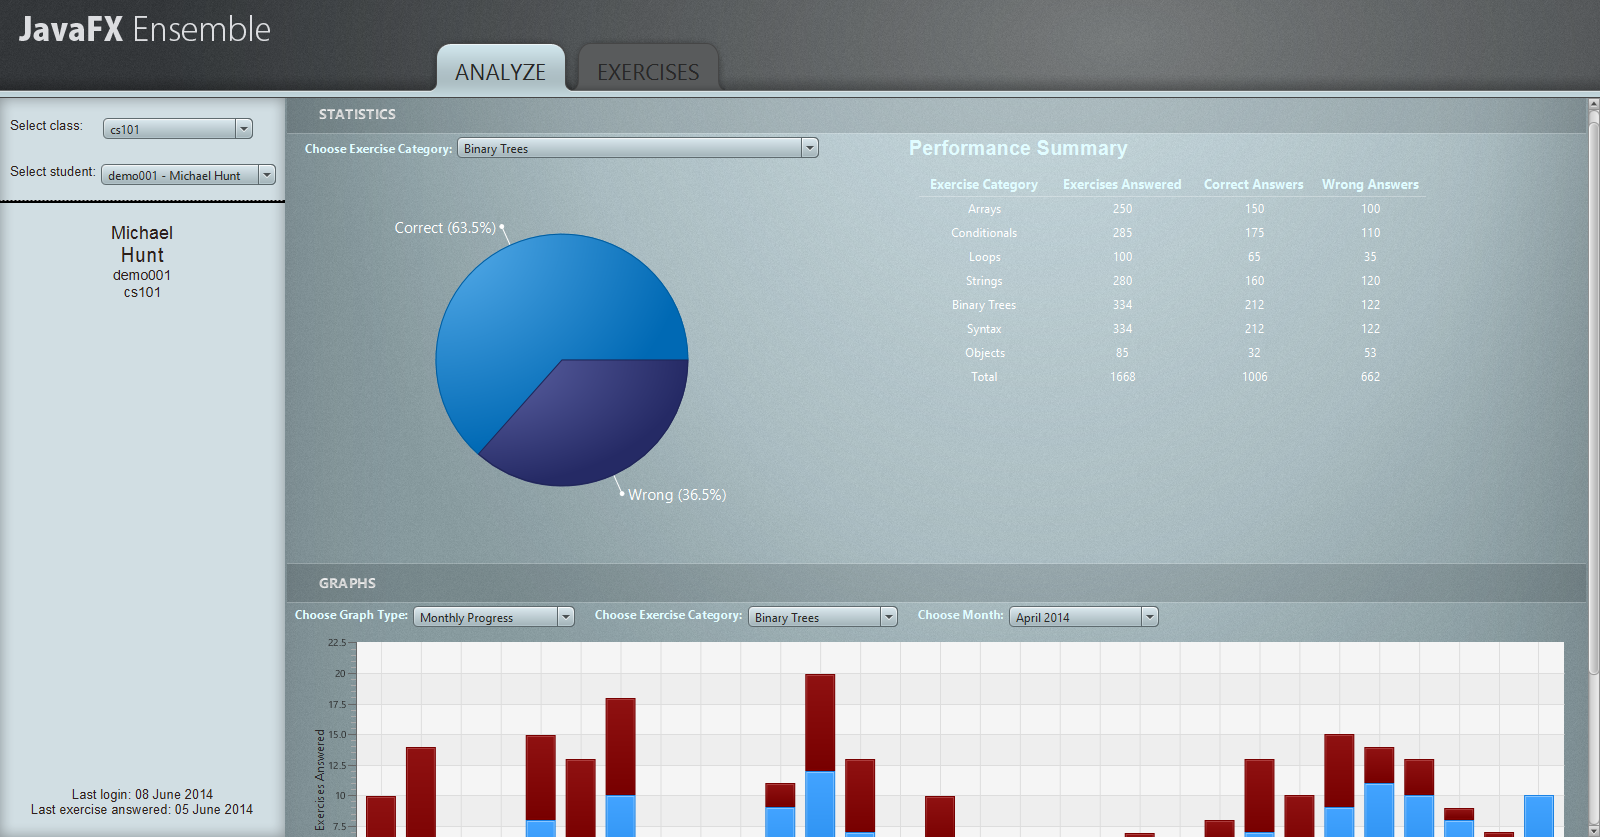
\includegraphics[width=\textwidth,height=\textheight,keepaspectratio]{analyze_overview}
\caption{An overview of the Analyze tab in the jSCAPE admin tool.}
\label{fig:analyze_overview}
\end{figure}

The jSCAPE admin tool provides teachers with the ability to track student progress and performance over time. Figure \ref{fig:analyze_overview} gives an overview of the Analyze tab, where statistical data about selected students can be displayed. The information displayed is identical to that displayed in the jSCAPE Profile tab (section \ref{subsec:tracking-progress}). On the left hand side of the window, the light blue box contains options to filter which data is displayed in the main window. A close up of the filter options is shown in figure \ref{fig:analyze_select_student}.

\begin{figure}[H]
\centering
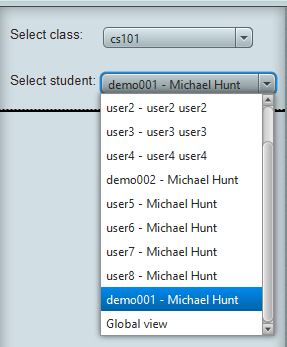
\includegraphics[scale=1]{analyze_select_student}
\caption{Selection possibilities in the Analyze tab.}
\label{fig:analyze_select_student}
\end{figure}

The jSCAPE system includes support for multiple classes to allow for both the separation of students and the separation of exercises available to a class. A teacher can select a class to view statistics about those students taking the class. This will update the list of students in the combo box, allowing the teacher to focus his attention on the performance of one particular student. \newline

Selecting a student will show their profile information in the light blue window, along with the date of their last login, and the date of their last exercise answered. In addition, the pie charts, performance table and progress graphs will be updated to reflect the performance of the selected student. Finally, there is an option to obtain a global view of the class' performance by selecting the ``Global view" option. 

\begin{figure}[H]
\centering
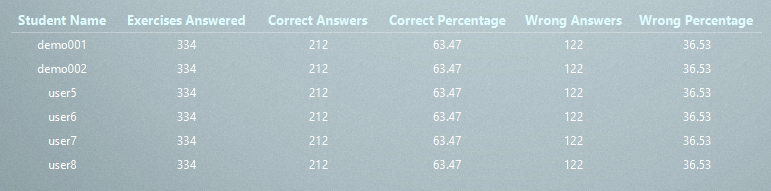
\includegraphics[width=\textwidth,height=\textheight,keepaspectratio]{global_view}
\caption{Global statistics view of a class.}
\label{fig:global_view}
\end{figure}

Figure \ref{fig:global_view} shows the table that is displayed after selecting the global view option. This table shows all the students who have answered exercises in a particular exercise category. In the example above, the data shown is for the ``Syntax" exercise category. The student user names are listed along with the number of exercises they have answered, and a detailed breakdown of the number of correct and wrong answers in terms of raw values and percentages. \newline

There is a combo box to select which exercise category to display, but this isn't shown in the picture to minimize the size of it. The global view feature is useful for teachers to identify which students may be facing difficulties. They can then select the student in the Analyze tab to get more detailed statistics and information about the student's progress.

\subsection{Managing the exercise bank}
\subsubsection{Managing exercise categories}
add description, lecture links and helpful links

\subsubsection{Adding an exercise manually}
add exercise manually

\subsubsection{Automatically generating exercises}
runs the appropriate exercise generator and stores the exercises in the database.


\section{Summary}
In this section we gave an overview of the components present in the jSCAPE system. 

We showed that jSCAPE performed a lot of tracking of student's performances by storing useful statistics concerning their progress. In addition\newline

In the following chapter, we talk more about the design of the system and various interesting implementation details and difficulties faced during the development of this project.

